\documentclass[11pt,a4paper]{article}

% --- Pakete ---
\usepackage[ngerman]{babel}
\usepackage[utf8]{inputenc}
\usepackage[T1]{fontenc}
\usepackage{lmodern} % Computer Modern (empfohlen)
\usepackage{geometry}
\geometry{
  a4paper,
  left=2.5cm,
  right=2.5cm,
  top=2.5cm,
  bottom=2.5cm
}
\usepackage{setspace}
\setstretch{1.24} % entspricht Empfehlung (1–1.5 Zeilenabstand)
\usepackage{microtype}
\usepackage{csquotes}
\usepackage{amsmath,amssymb}
\usepackage{graphicx}
\usepackage{caption}
\usepackage{subcaption}
\usepackage{siunitx}     % saubere Einheiten, Einheiten aufrecht
\sisetup{detect-all}
\usepackage{booktabs}
\usepackage{hyperref}
\usepackage{enumitem}
\usepackage{subcaption}
\def\UrlBreaks{\do\/\do-} % Erlaubt Zeilenumbrüche in URLs nach / und -

\usepackage{fancyhdr}
\usepackage{mhchem}

% --- Kopf- und Fußzeile ---
\pagestyle{fancy}
\fancyhf{}
\fancyfoot[C]{\thepage}
\renewcommand{\sectionmark}[1]{%
  \markboth{\thesection\ #1}{}%
}


% --- Nummerierte Gleichungen ---
\numberwithin{equation}{section}

% --- Abbildungs- und Tabellenbeschriftungen ---
\captionsetup{font=small,labelfont=bf}


% --- Metadaten (für Titelseite) ---
\newcommand{\Lehrveranstaltung}{Praktikum Physikalische Eigenschaften der Materialien}
\newcommand{\Universitaet}{Universität Augsburg}
\newcommand{\Semester}{Wintersemester 2025/2026}
\newcommand{\Versuchsnummer}{5}
\newcommand{\Versuchstitel}{Korrosion}
\newcommand{\Gruppe}{C}
\newcommand{\Versuchsdatum}{04.03.2026}
\newcommand{\Abgabedatum}{TT.MM.JJJJ}
\newcommand{\Abgabeart}{Gemeinsames Versuchsprotokoll}
\newcommand{\Autor}{Fabio Piskorz, Fabio Nogielsky, Konstantin Szantho von Radnoth }

% ---------------------------------------------------
% Titelseite (ohne Seitenzahl)
% ---------------------------------------------------
\begin{document}
\pagenumbering{gobble} % keine Seitenzahl auf Titelseite

\begin{titlepage}
    \centering
    {\Large \Lehrveranstaltung\par}
    \vspace{0.5cm}
    {\large \Universitaet\par}
    \vspace{0.5cm}
    {\large \Semester\par}
    \vspace{1.5cm}
    {\Large Versuchsnummer: \Versuchsnummer\par}
    \vspace{0.5cm}
    {\Large Versuchstitel: \Versuchstitel\par}
    \vspace{1.5cm}
    {\large Gruppe \Gruppe\par}
    \vspace{0.5cm}
    {\LARGE \Abgabeart\par}
    \vspace{0.5cm}
    {\large Autor(en): \Autor\par}
    \vspace{1.5cm}
    {\large Versuchsdatum: \Versuchsdatum\par}
    \vspace{0.5cm}
    {\large Abgabedatum: \Abgabedatum\par}

    \vfill
\end{titlepage}


%Inhaltsverzeichnis
\tableofcontents
\newpage
% ab hier Seitenzahlen normal
\pagenumbering{arabic}

\section{Einleitung}

Materialien sind im Alltag permanent verschiedensten Umwelteinflüssen ausgesetzt. Sei es die Autokarosserie, die Regen und winterlichem Streusalz standhalten muss, der Rumpf eines Schiffes im Meerwasser oder auch das alltägliche Silberbesteck in der Spülmaschine. Führt die Reaktion eines metallischen Werkstoffs mit seiner Umgebung zu einer messbaren Veränderung und zu einer Beeinträchtigung seiner Funktion, so wird dies als Korrosion bezeichnet \cite{korrosioDef}. Am geläufigsten ist hierbei das Rosten von Eisenwerkstoffen. Prinzipiell lassen sich diese Schädigungen auf chemische, elektrochemische, physikalische oder biologische Ursachen zurückführen.

\noindent Die Relevanz dieses Themas zeigt sich nicht nur beim ärgerlichen Rostfleck an der Fahrradkette, sondern vor allem in der globalen Wirtschaft und Sicherheit. Jährlich entstehen weltweit Schäden in Milliardenhöhe durch korrodierte Rohrleitungen, marode Brücken oder ausfallende Industrieanlagen \cite{nace_impact_2016}. Korrosion ist somit nicht nur ein optisches Problem, sondern ein massiver wirtschaftlicher Faktor und ein potenzielles Sicherheitsrisiko.
\noindent Um diese weitreichenden Schäden zu verhindern, müssen die zugrundeliegenden Mechanismen verstanden und quantifiziert werden.

\section{Theorie}

\subsection{Grundlagen der Korrosion}
Während die Korrosion in heißen Gasen auf direkter Oxidation ohne Elektrolyt basiert und meist diffusionskontrollierten Wachstumsgesetzen gehorcht \cite{tostmann2001korrosion}, beschränkt sich dieser Versuch auf die elektrochemische Korrosion. Diese findet in wässrigen Medien (Elektrolyten) statt und strebt ein thermodynamisches Minimum an, welches durch eine negative Änderung der freien Enthalpie ($\Delta G < 0$) gekennzeichnet ist. 

\subsection{Elektrochemische Thermodynamik}
Bei der elektrochemischen Korrosion stellt sich an der Phasengrenze zwischen Metall und Elektrolyt ein dynamisches Gleichgewicht ein, bei dem das Metall sich auflädt. Das sich dabei aufbauende Potenzial $U$ lässt sich über die Nernstsche Gleichung beschreiben:
\begin{equation}
    U = U_0 - \frac{R T}{n F} \cdot \ln\left([Me^{n+}]\right)
    \label{eq:nernst}
\end{equation}
Dabei ist $U_0$ das Standardpotenzial, $R$ die universelle Gaskonstante, $T$ die Temperatur, $n$ die Wertigkeit der Ionen und $F$ die Faraday-Konstante. Da absolute Einzelpotenziale nicht messbar sind, wird als Bezugspunkt die Standardwasserstoffelektrode ($U_0 = \qty{0}{\volt}$) definiert. In der resultierenden elektrochemischen Spannungsreihe gelten Metalle mit positivem Potenzial gegenüber diesem Nullpunkt als edel, solche mit negativem als unedel. 

\noindent Thermodynamische Stabilitätsbereiche, in denen das Metall immun, aktiv korrodierend oder passiviert vorliegt, lassen sich in Pourbaix-Diagrammen in Abhängigkeit des pH-Wertes darstellen. Sie erlauben jedoch keine Aussage über die tatsächliche Reaktionsgeschwindigkeit \cite{barthelgrenzen}.

\subsection{Kinetik und Reaktionsgeschwindigkeit}
Das Maß für die korrodierte Stoffmenge pro Zeiteinheit lässt sich durch das erste und zweite Faradaysche Gesetz \cite{lupke1899faradaysche} direkt mit dem fließenden Strom $I$ verknüpfen:
\begin{equation}
    \frac{\Delta m}{\Delta t} = \frac{I \cdot M_0}{z \cdot F}
    \label{eq:faraday}
\end{equation}
Hierbei beschreibt $M_0$ die molare Masse und $z$ die Wertigkeit. Um den Einfluss der Probengeometrie auszuschließen, wird standardmäßig die flächenbezogene Stromdichte $i = I/A$ betrachtet.

\noindent Weicht eine Elektrode von ihrem Gleichgewichtspotenzial $E_R$ ab, spricht man von der Überspannung $\eta$. Die resultierende Stromdichte wird maßgeblich vom langsamsten Teilschritt der Reaktion limitiert:
\begin{itemize}
    \item \textbf{Durchtrittskontrolle:} Ist der Ladungsdurchtritt vom Anodenmaterial in den Elektrolyten der geschwindigkeitsbestimmende Schritt, folgt die Übertrittsgeschwindigkeit dem Arrhenius-Gesetz ($k = k_0 \cdot \exp(-\frac{E_A}{RT})$), wobei die Aktivierungsenergie $E_A$ vom elektrischen Feld abhängt. Die Gesamtstromdichte $i$ ergibt sich aus der Summe von anodischer ($i_a$) und kathodischer ($i_k$) Teilstromdichte in Abhängigkeit der Überspannung $\eta$:
    \begin{equation}
        i = i_a + i_k = i_0 \cdot \left[ \exp\left(\frac{\alpha n F \eta}{R T}\right) - \exp\left(-\frac{(1-\alpha) n F \eta}{R T}\right) \right]
        \label{eq:butlervolmer}
    \end{equation}
    Hierbei ist $i_0$ die Austauschstromdichte und $\alpha \in [0;1]$ der Durchtrittsfaktor (meist $\alpha \approx 0,5$). Am Gleichgewichtspotenzial ($\eta = 0$) finden beide Reaktionen gleich schnell statt, sodass $i_0 = i_a = -i_k$ gilt und makroskopisch kein Strom fließt.
    
\noindent Im Bereich sehr kleiner Überspannungen ($|\eta| < \qty{0,017}{\volt}$) lässt sich die Funktion linearisieren ($i \approx i_0 \frac{n F}{R T} \eta$). Aus dem Kehrwert dieser Steigung ergibt sich der Polarisationswiderstand $r$:
    \begin{equation}
        r = \frac{R T}{n F \cdot i_0}
        \label{eq:polwiderstand}
    \end{equation}
 \noindent Für große Überspannungen ($|\eta| \gg 0$) verschwindet entweder der anodische oder kathodische Anteil. Dies führt zum logarithmischen Verhalten der Tafel-Gleichung:
    \begin{equation}
        \ln|i| = \ln(i_0) + \beta \cdot \eta
        \label{eq:tafel}
    \end{equation}
\noindent mit dem  Anstiegsfaktor $\beta$ = $\frac{\alpha nF}{RT}$ f\"ur $\eta$ > 0, und $\beta$ = $-\frac{(1-\alpha) nF}{RT}$ f\"ur $\eta$ <  0.
    
    \item \textbf{Diffusionskontrolle:} Ist hingegen der Stofftransport zur Elektrode limitiert, nähert sich die Stromdichte für hohe Überspannungen asymptotisch einer maximalen Grenzstromdichte $i_{gr}$ an.
\end{itemize}

\subsection{Mischelektroden und Passivierung}
In einer realen Korrosionszelle (Mischelektrode) stellt sich das Ruhe- oder Korrosionspotenzial $E_{korr}$ ein. An diesem Potenzial heben sich der anodische Teilstrom $i_a$ und der kathodische Teilstrom $i_k$ exakt auf, wodurch die Zelle nach außen hin stromlos erscheint ($i_a + i_k = 0$). 

\noindent Bei unedlen Metallen kann es bei zunehmender anodischer Belastung zur Passivierung kommen. Überschreitet die anodische Stromdichte einen kritischen Wert, kristallisiert lokal eine schützende Deckschicht aus. Der Korrosionsstrom bricht in diesem Bereich drastisch ein, bis das angelegte Potenzial stark genug ist, um die schützende Passivschicht wieder aufzubrechen.

\subsection{Das Belüftungselement}
Wie sich aus der Nernst-Gleichung \ref{eq:nernst} herleiten lässt, hängt das Potenzial einer Elektrode nicht nur vom Metall selbst, sondern auch von im Elektrolyten gelösten Gasen ab. Ein wesentlicher Mechanismus der lokalen Korrosion, der sich daraus ergibt, ist das Belüftungselement nach Evans. Taucht ein Werkstück in einen Elektrolyten mit lokal unterschiedlicher Sauerstoffkonzentration, entsteht ein Lokalelement auf demselben Metall. Bereiche mit hoher Sauerstoffzufuhr (wie der Rand eines Wassertropfens) wirken kathodisch. Sauerstoffarme Bereiche (z.\,B.\ in Spalten oder im Zentrum des Tropfens) werden hingegen zur Anode und gehen unter Materialauflösung in Lösung. Dieses Prinzip ist die treibende physikalische Kraft hinter der Spalt- und Tropfenkorrosion.


\section{Versuchsbeschreibung}


\subsection{Elektrochemische Spannungsreihe}

\begin{figure}[ht]
\centering

\includegraphics[width=0.7\textwidth]{elektrischeSR.jpeg}
\caption{Aufbau der elektrischen Spannungsreihe}
\label{fig:elSR}
\end{figure}
\noindent F\"ur die Versuche werden zwei Zink, zwei Kupfer, sieben Eisen und ein Edelstahl Stab ben\"otigt.

\noindent Zur Vorbereitung werden die Proben geschliffen und poliert, um sie von vorherigen Korrosionsr\"uckst\"anden zu befreien und um ihre Oberfl\"ache m\"oglichst Eben zu bekommen, damit die sp\"ateren Reaktionsergebnisse vergleichbar sind.
Die elektrochemische Spannungsreihe wird mit folgenden Probenpaaren aufgebaut:
\newpage
\begin{enumerate}[label = \alph*)]
\item \ce{Fe} -- \ce{Cu} ohne elektrischen Kontakt
\item \ce{Fe} -- \ce{Zn} ohne elektrischen Kontakt
\item \ce{Fe} -- \ce{Zn} mit elektrischen Kontakt
\item \ce{Fe} -- \ce{Cu} mit elektrischen Kontakt
\label{list:elSp}
\end{enumerate}



\noindent Die Paare werden jeweils in eine Glasschale gelegt und mit Kochsalzl\"osung (\ce{NaCl}) bedeckt. Es wird dabei darauf geachtet, dass die Proben sich nicht gegenseitig ber\"uhren.
\noindent Die verbleibenden Paare c) und d) werden zus\"atzlich mithilfe von Krokodilsklemmen elektrisch miteinander verbunden. Hierbei ist darauf zu achten, dass die Klemmen m\"oglichst keinen Kontakt zur L\"osung haben, um eine Kontaktkorrosion an dieser Stelle zu vermeiden. Der gesamte Aufbau (Abb. \ref{fig:elSR}) findet unter dem Abzug statt. Der Versuch wird zu Anfang des Praktikums aufgebaut und bis zum Ende stehen gelassen.

\subsection{Korrosionsmesszelle}

\begin{figure}[ht]
\centering
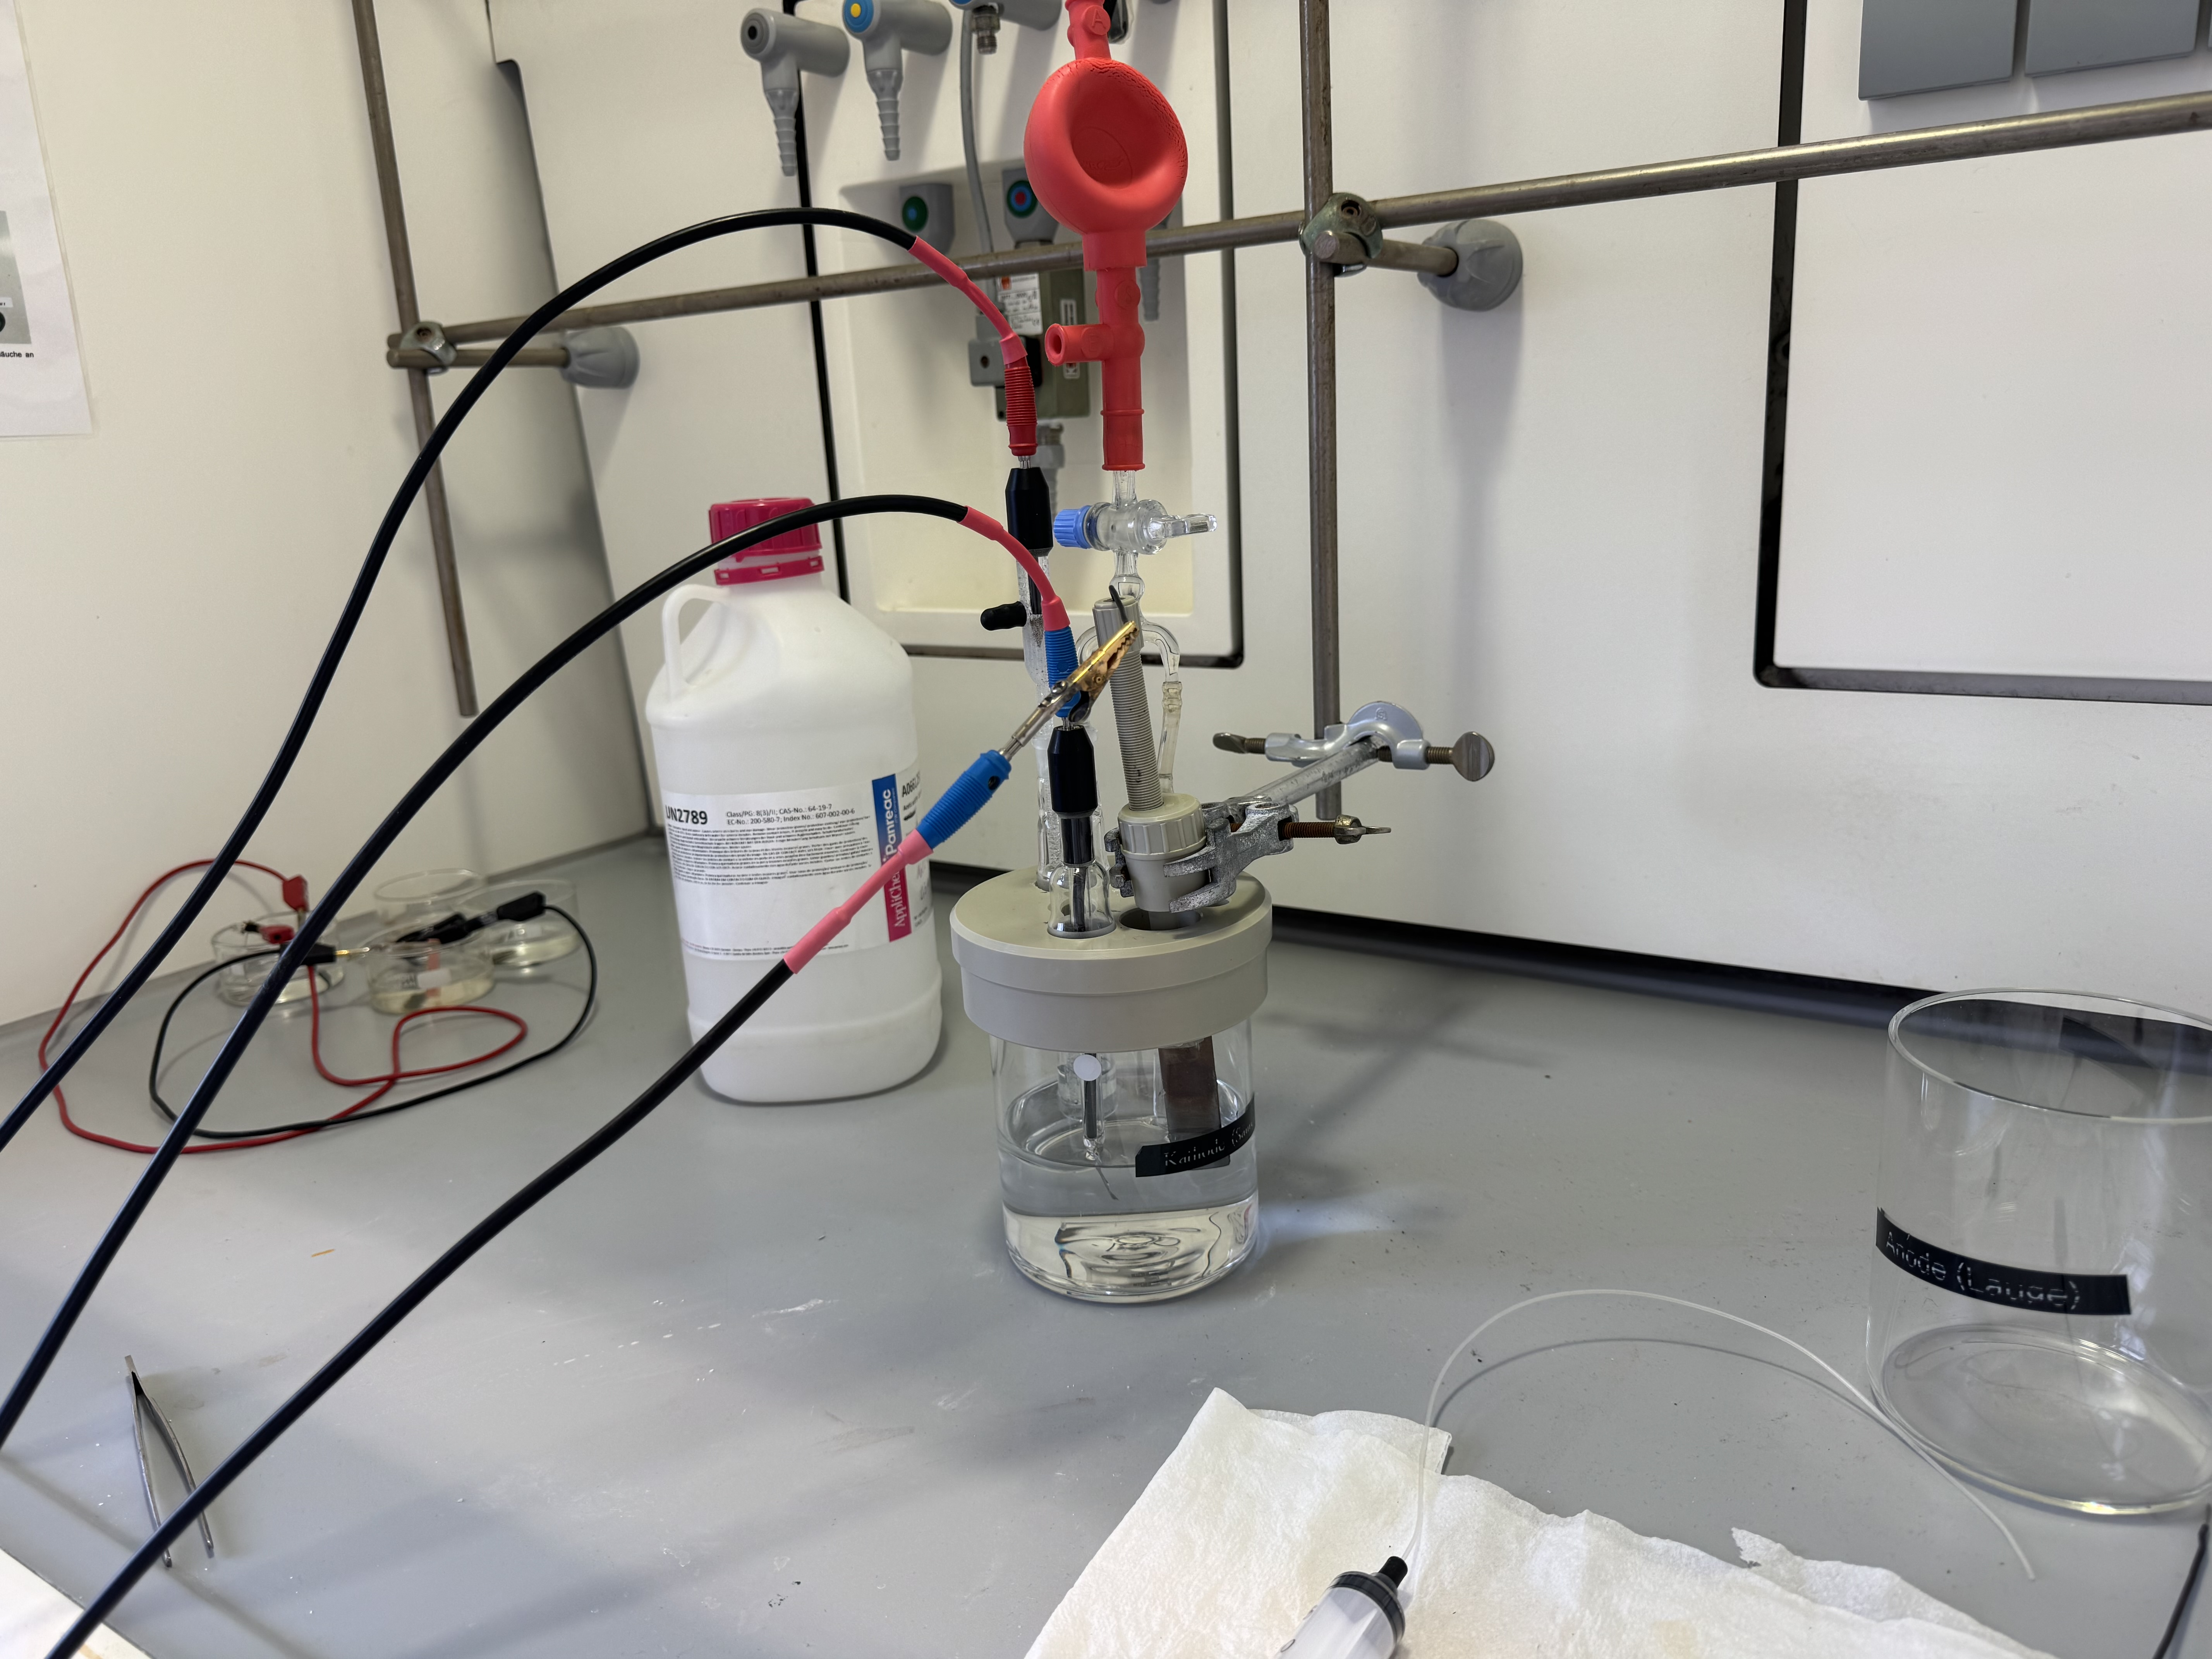
\includegraphics[width=0.7\textwidth]{Korrosionsmesszelle.jpeg}
\caption{Aufbau der Korrosionsmesszelle}
\label{fig:krMZ}
\end{figure}

\noindent Die Korrosionsmesszelle (Abb. ~\ref{fig:krMZ}) besteht aus einem Hauptgef\"a{\ss}, welches mit Elektrolyt bef\"ullt ist und einem Deckel mit \"Offnungen f\"ur alle Messger\"ate. Das Zwisschengef\"a{\ss} wird mittels einer Pipette mit Pipettierballon mit ca. 15 ml Elektrolyt bef\"ullt. Mithilfe eines Stromschl\"ussels  wird eine Verbindung zwischen Referenzgef\"a{\ss} und dem Hauptgef\"a{\ss}  hergestellt. Das gerade St\"uck des Stromschl\"ussels wird mithilfe einer Spritze und einem d\"unnen Schl\"auch vollst\"andig mit Elektrolyt zu bef\"ullt. Dabei wird darauf geachtet, dass sich keine Luftblasen bilden. Der andere Zweig besteht aus einer Halber-Luggin-Kapilare und muss auch mit Elektrolyt bef\"ullt werden, hierzu wird der Pipettierballon an der oberen \"Offnung des Stromschl\"ussels angesetzt und das Elektrolyt durch die Kapillare hochgezogen bis die Verbindung beider Zweige gef\"ullt ist. Die Probenhalterung wird ca. 1 cm in die L\"osung geh\"angt 
\newline Abschlie{\ss}end werden die Gegen- und Referenzelektrode eingesetzt. Gemeinsam mit der Arbeitselektrode, also der Probe,  mit einem Netzger\"at verbunden.
Der Versuch wird f\"ur zwei Verschiede Proben, zwei Elektolyte und bei zwei Temperaturen durchgef\"uhrt.
\begin{enumerate}[label = \Alph*)]
\item \ce{Fe} in \ce{NaCl} bei $T_{\text{Raum}} \approx \qty{23}{\degreeCelsius}$
\item \ce{Fe} in \ce{H2SO4} (verd\"unnt) bei $T_{\text{Raum}}$
\item \ce{Fe} in \ce{H2SO4} (verd\"unnt) bei $T_{\text{erw\"ahrmt}} \approx \qty{30}{\degreeCelsius}$ 
\item Chromstahl in \ce{H2So4} (verd\"unnt) bei $T_{\text{Raum}}$
\end{enumerate}
Die Proben besitzen jeweils eine Fl\"ache von $A_{\text{Probe}} \approx \qty{150}{\milli\metre\squared}$. Sie werden vor dem Einsetzen von vorherigen R\"uckst\"anden befreit.
Die Versuche mit erw\"ahrmten Elektrolyt werden auf einer Heizplatte unter st\"andigem R\"uhren (mittels eines magnetischen R\"uhrfischchens) durchgef\"uhrt.

\subsection{Aufnahme der Stromdichte-Porenzial-Kurve}
Die Kennlinie wird mithilfe eines Potentiostats und einer Software am Computer aufgenommen. Vor Versuchsbeginn wird sich mit der Funktionsweise vertraut gemacht. 
Die Messsoftware ben\"otigt $A_{\text{Probe}}$ als Messparamter einegtragen, der Potentialbereich wird Schrittweise durchfahren. 
Vor Messbeginn wird gewartet bis sich das Ruhepotenzial $\phi_{\text{Ruhe}}$ stabilisiert hat. Es wird notiert und die Messung wird gestartet.

\newpage
\section{Auswertung und Diskussion}

\subsection{Elektrochemische Spannungsreihe}

\begin{figure}[ht]
\centering

\includegraphics[width=0.7\textwidth]{SRende.jpeg}
\caption{Korrosion an den Proben der Spannungsreihe}
\label{fig:SRende}
\end{figure}

\noindent Gemäß der Nernst-Gleichung (Gl.~\ref{eq:nernst}) ergeben sich gegenüber der Standardwasserstoffelektrode die Standardpotenziale $U_{\text{0,Cu}} = \qty{+0,34}{\volt}$, $U_{\text{0,Fe}} = \qty{-0,41}{\volt}$ und $U_{\text{0,Zn}} = \qty{-0,76}{\volt}$ \cite{chemiede_spannungsreihe}. 
Demnach lassen sich die verwendeten Proben von edel nach unedel wie folgt aufreihen:
\begin{equation*}
    \text{Cu} \ > \ \text{Fe} \ > \ \text{Zn}
\end{equation*}

%\noindent Werden zwei Metalle in einem Elektrolyten elektrisch leitend verbunden, entsteht ein kurzgeschlossenes Lokalelement. Dabei fungiert stets das unedlere Metall als Anode und geht unter Elektronenabgabe in Lösung (Oxidation). Das edlere Metall wirkt als Kathode, an der eine Reduktion (z.\,B.\ von Sauerstoff) stattfindet, ohne dass sich das Metall selbst auflöst.
\noindent Bei der Paarung aus Eisen und Kupfer \textbf{a)} verhält sich das edle Kupfer im verwendeten Elektrolyten thermodynamisch stabil und zeigt keine Anzeichen einer Oxidation. Das unedlere Eisen hingegen korrodiert unter Elektronenabgabe. Dies zeigt sich optisch in einer schwachen Trübung beziehungsweise einer braun-orangen Ausfällung (Eisen(III)-hydroxid) in direkter Nähe des Eisenblechs. Bei der Paarung aus Eisen und Zink ohne Kontakt \textbf{b)} oxidieren ebenfalls beide Metalle für sich allein. Da die in Lösung gehenden Zinkionen farblos sind, zeigt sich hier optisch jedoch nur eine leichte Ausfällung an der Eisenprobe (Abb. \ref{fig:SRende}).

\noindent Werden die Metalle elektrisch verbunden, bilden sich Lokalelemente, wodurch das Korrosionsverhalten nun direkt vom Standardpotenzial der Partner abhängt. Bei der Paarung aus Eisen und Zink mit Kontakt \textbf{c)} fungiert das sehr unedle Zink als Anode ($\text{Zn} \rightarrow \text{Zn}^{2+} + 2\text{e}^-$). Die abgegebenen Elektronen fließen zum edleren Eisen, welches kathodisch polarisiert wird. An der Eisenoberfläche findet folglich nur noch die Reduktion des Sauerstoffs statt. Das Eisen bleibt optisch blank und wird durch das Zink vollständig vor der Rostbildung geschützt.
\noindent Bei der Kombination aus Eisen und Kupfer mit Kontakt \textbf{d)} kehren sich die Verhältnisse für das Eisen um. In dieser Paarung ist das Eisen das unedlere Metall gegenüber dem Kupfer und übernimmt die Rolle der Anode. Es gibt seine Elektronen an das edle Kupfer ab, welches als Kathode fungiert. Durch diesen Aufbau wird die Oxidation des Eisens drastisch beschleunigt. Experimentell bestätigt sich dies durch eine deutlich intensivere Trübung sowie Rostbildung rund um das Eisenblech, während das Kupfer unbeschadet bleibt (Abb. \ref{fig:SRvgl}).

\begin{figure}[t]
\centering
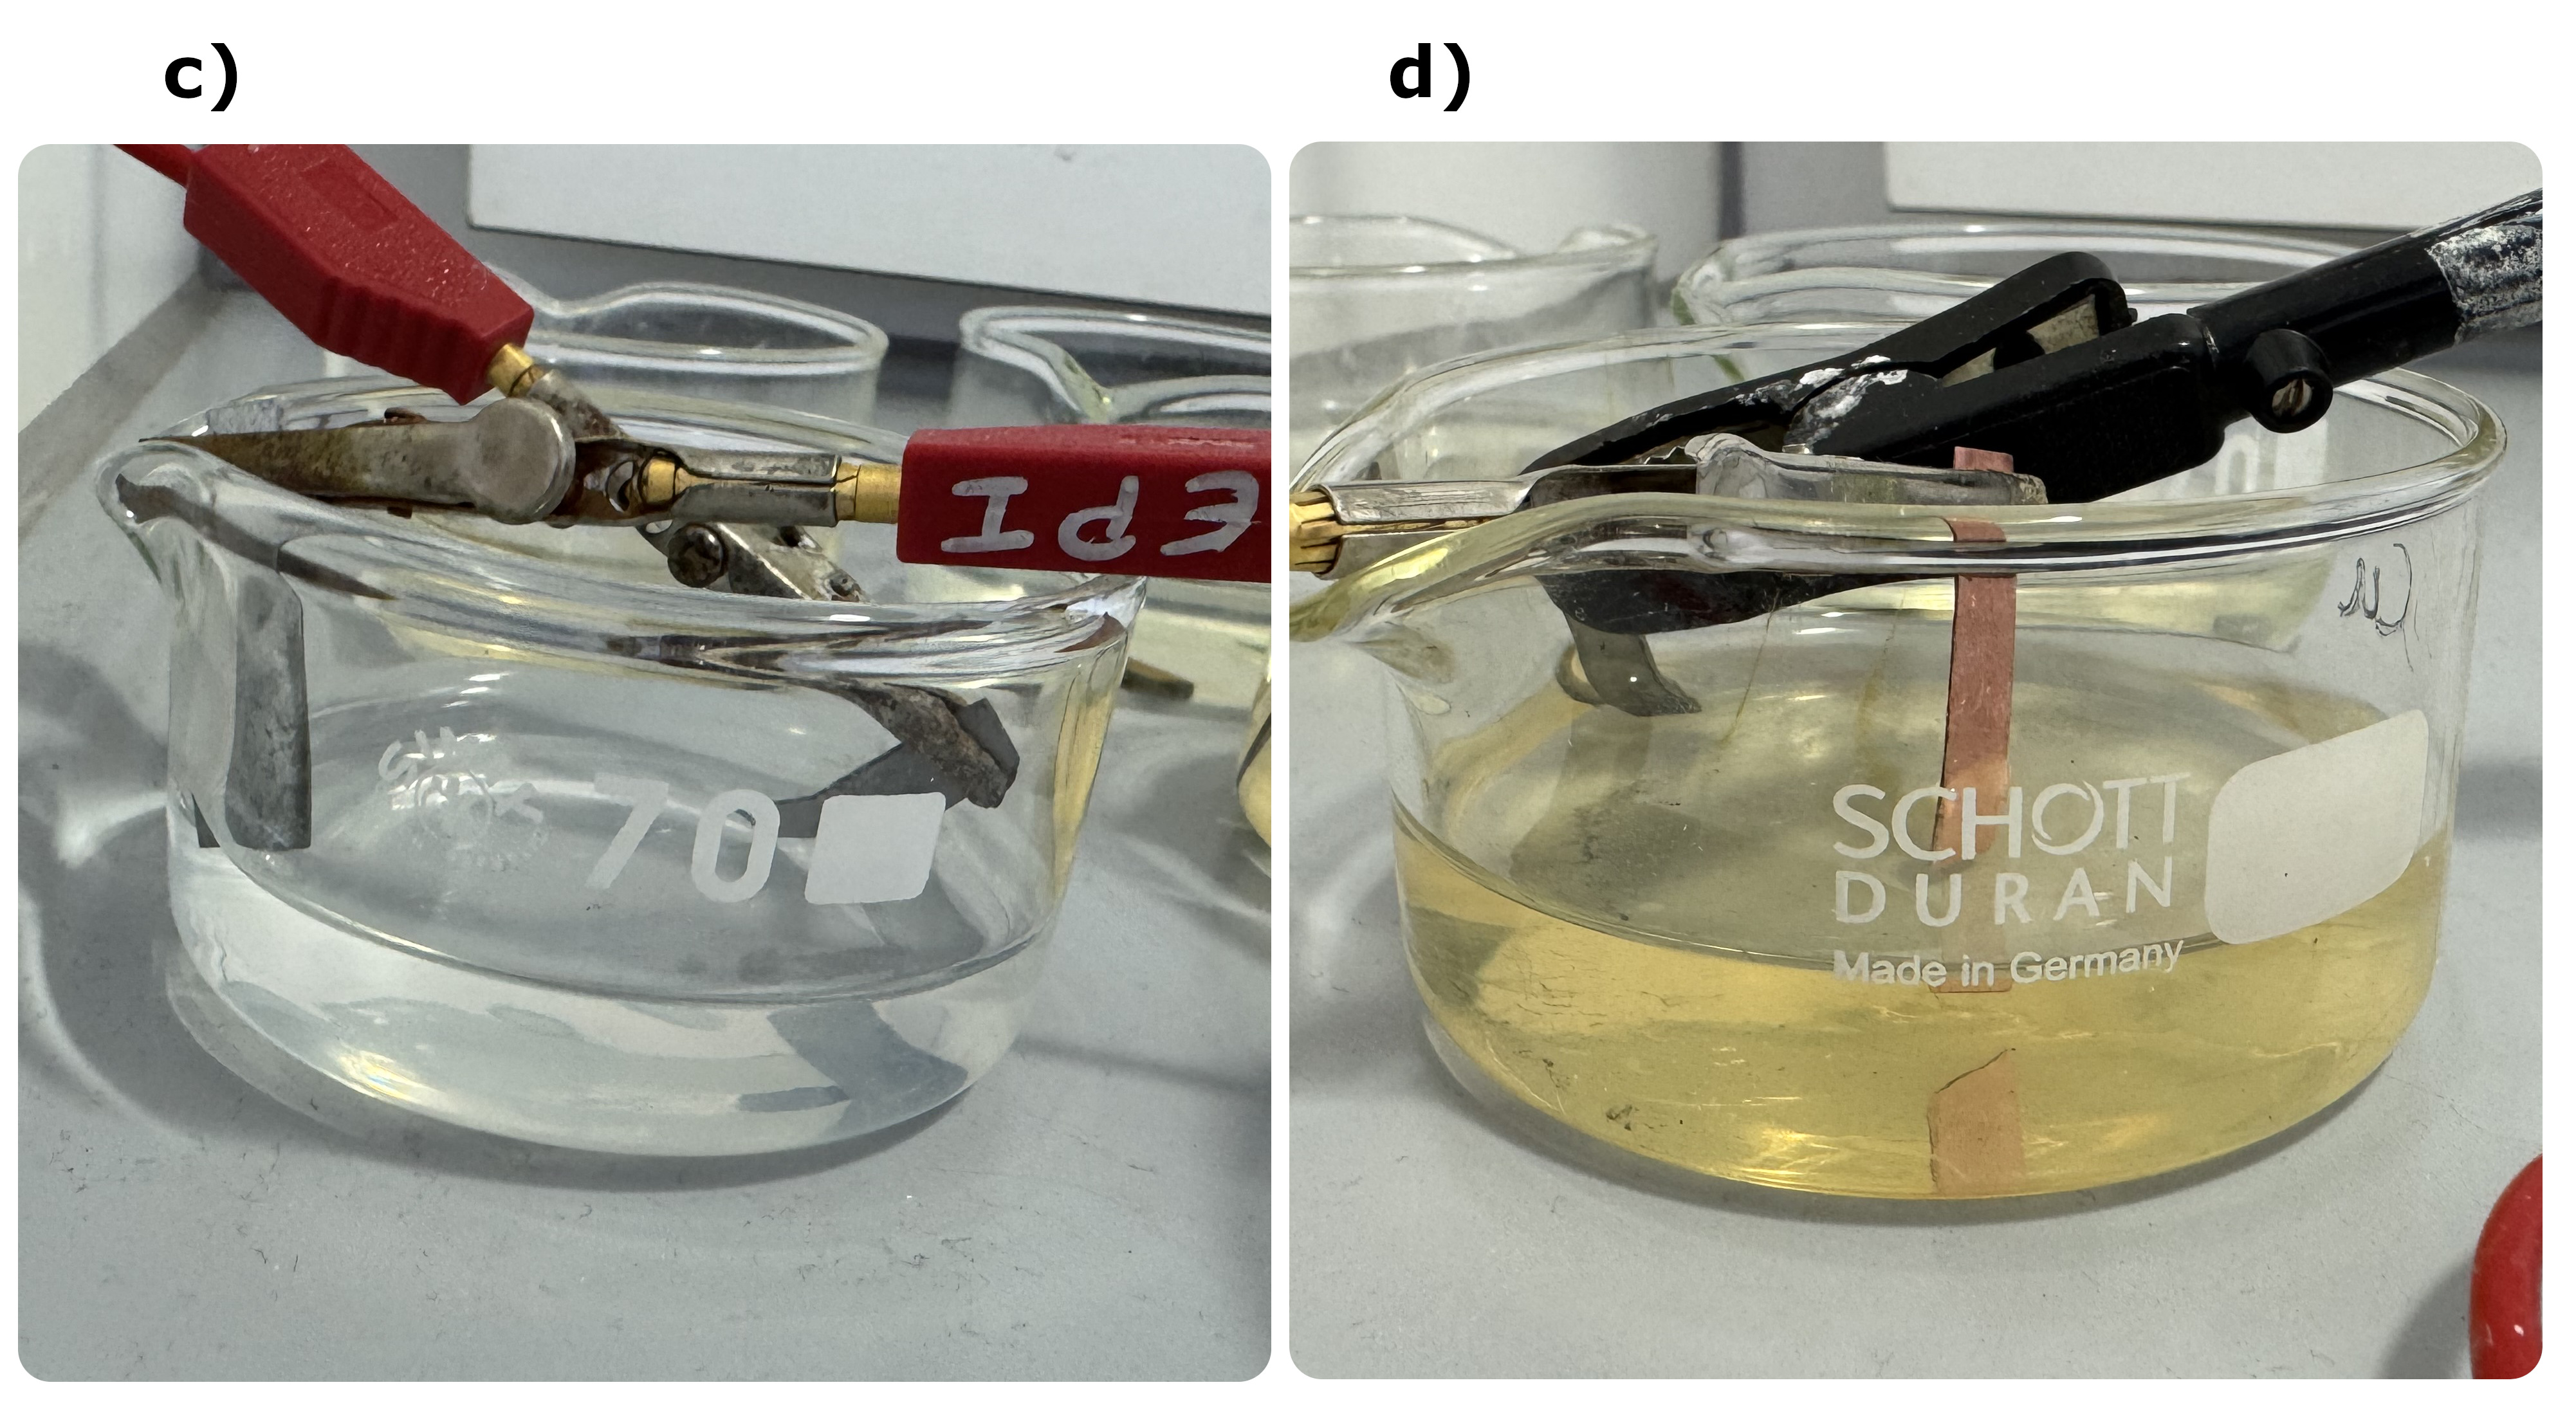
\includegraphics[width=0.7\textwidth]{srVergleich.jpeg}
\caption{Vergleich der Korrosion an den Proben c) und d)}
\label{fig:SRvgl}
\end{figure}

\subsection{Stromdichte-Porenzial-Kurven}


\begin{figure}[t]
    \centering
    % Erste Zeile: Plot A (links) und Plot D (rechts)
    \begin{subfigure}[b]{0.48\textwidth}
        \centering
        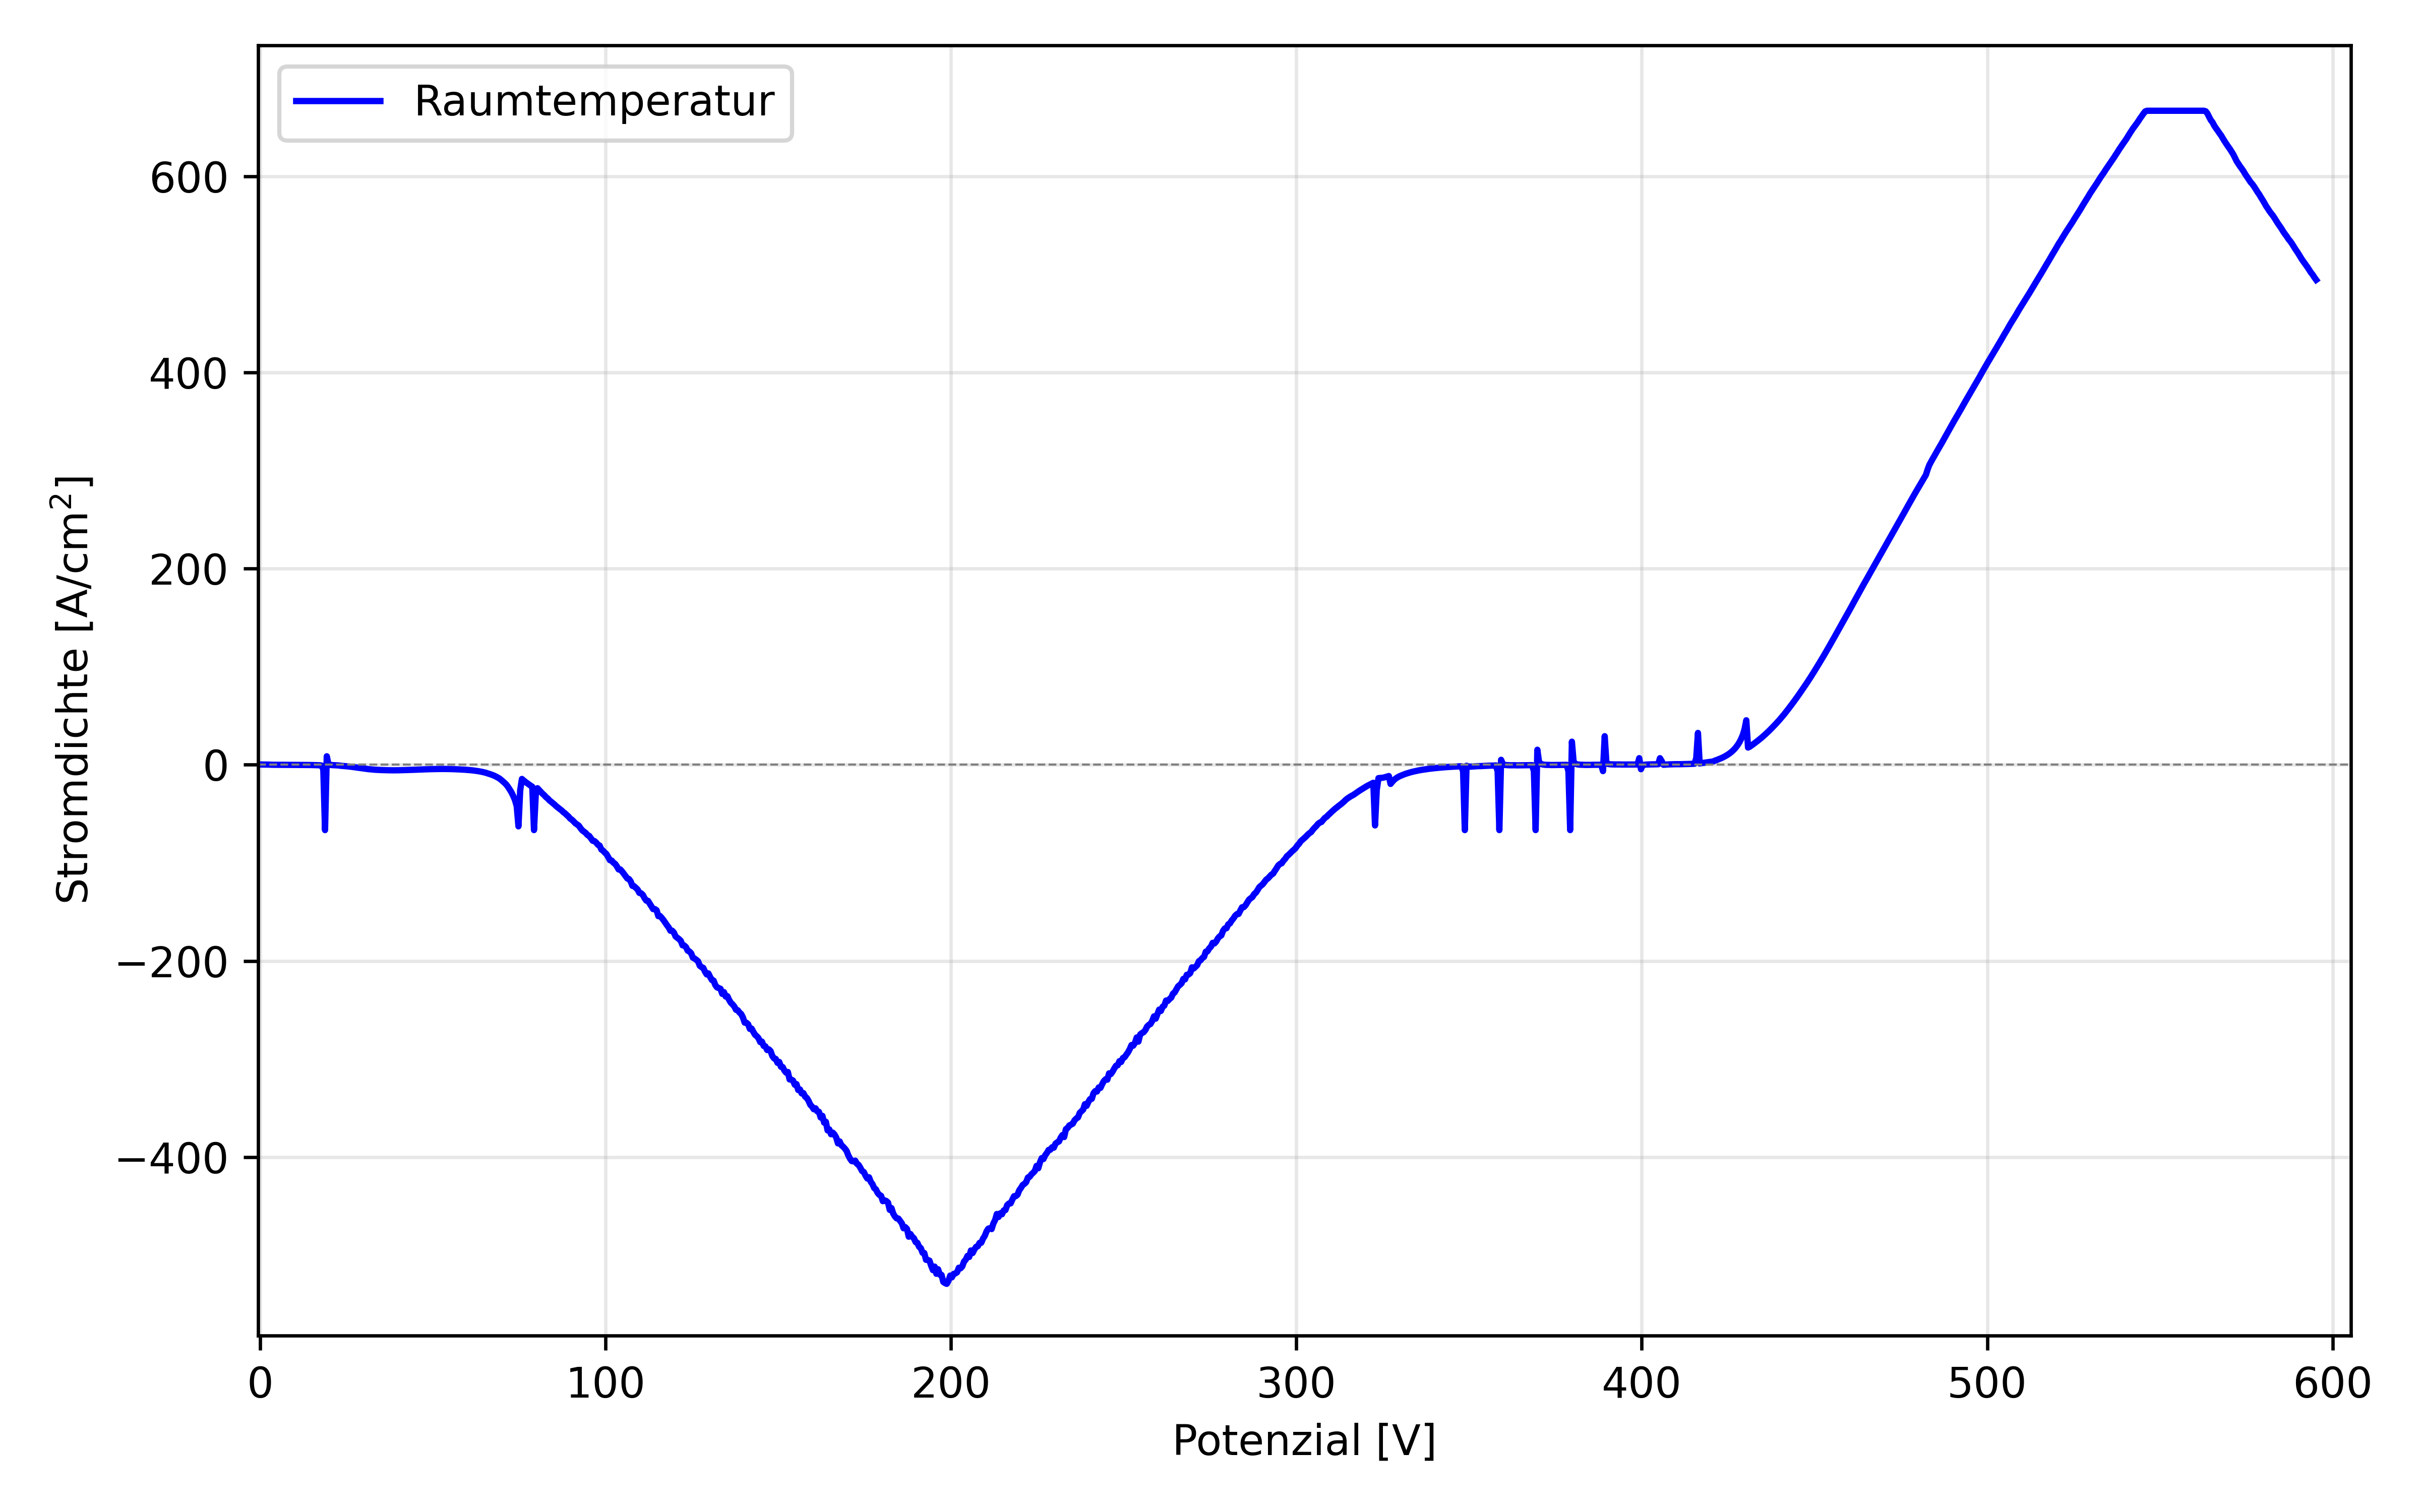
\includegraphics[width=\textwidth]{EIsen_in_NHCl(2)_plot.png} % Dateinamen anpassen!
        \caption*{A) Fe in NaCl bei Raumtemperatur}
        \label{fig:plot_A}
    \end{subfigure}
    \hfill
    \begin{subfigure}[b]{0.48\textwidth}
        \centering
        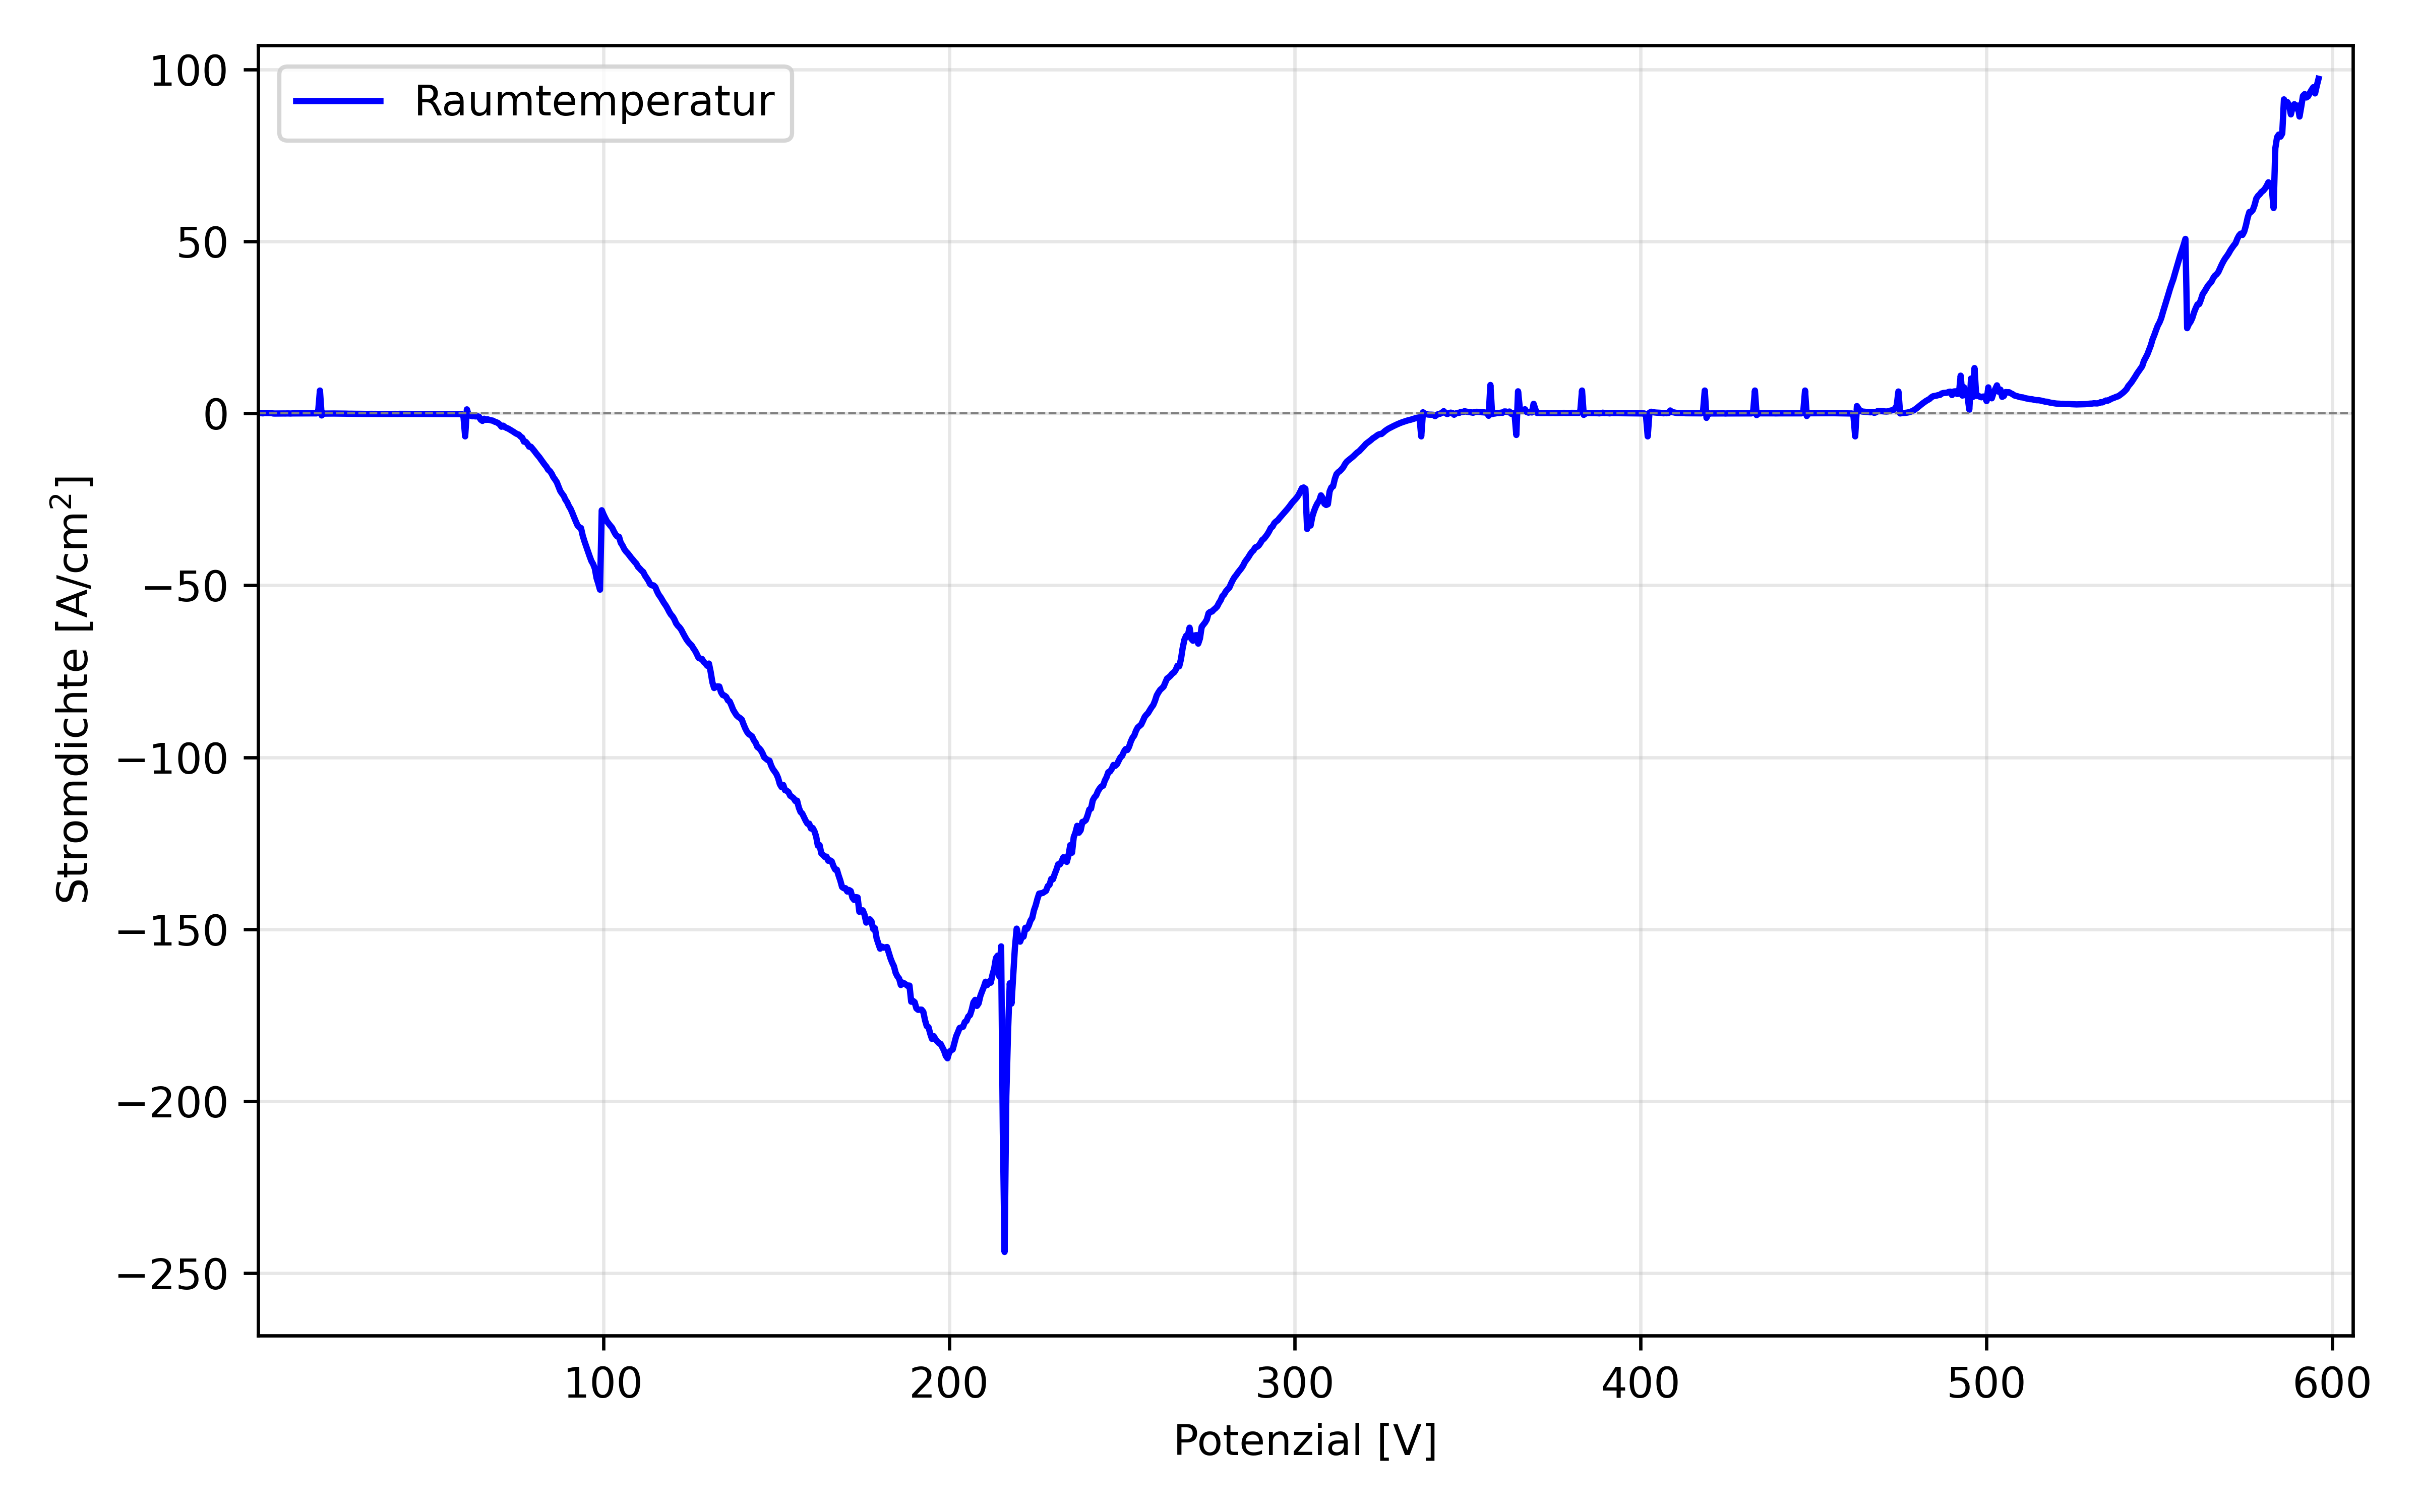
\includegraphics[width=\textwidth]{Chromstahl_in_H2So4_bei RT_plot.png} % Dateinamen anpassen!
        \caption*{D) Chromstahl in verd.\ $\text{H}_2\text{SO}_4$ bei RT}
        \label{fig:plot_D}
    \end{subfigure}
    
    \vspace{0.5cm} % Etwas Abstand zwischen den Zeilen
    
    % Zweite Zeile: Gemeinsamer Plot B & C (zentriert, etwas größer)
    \begin{subfigure}[b]{0.6\textwidth}
        \centering
        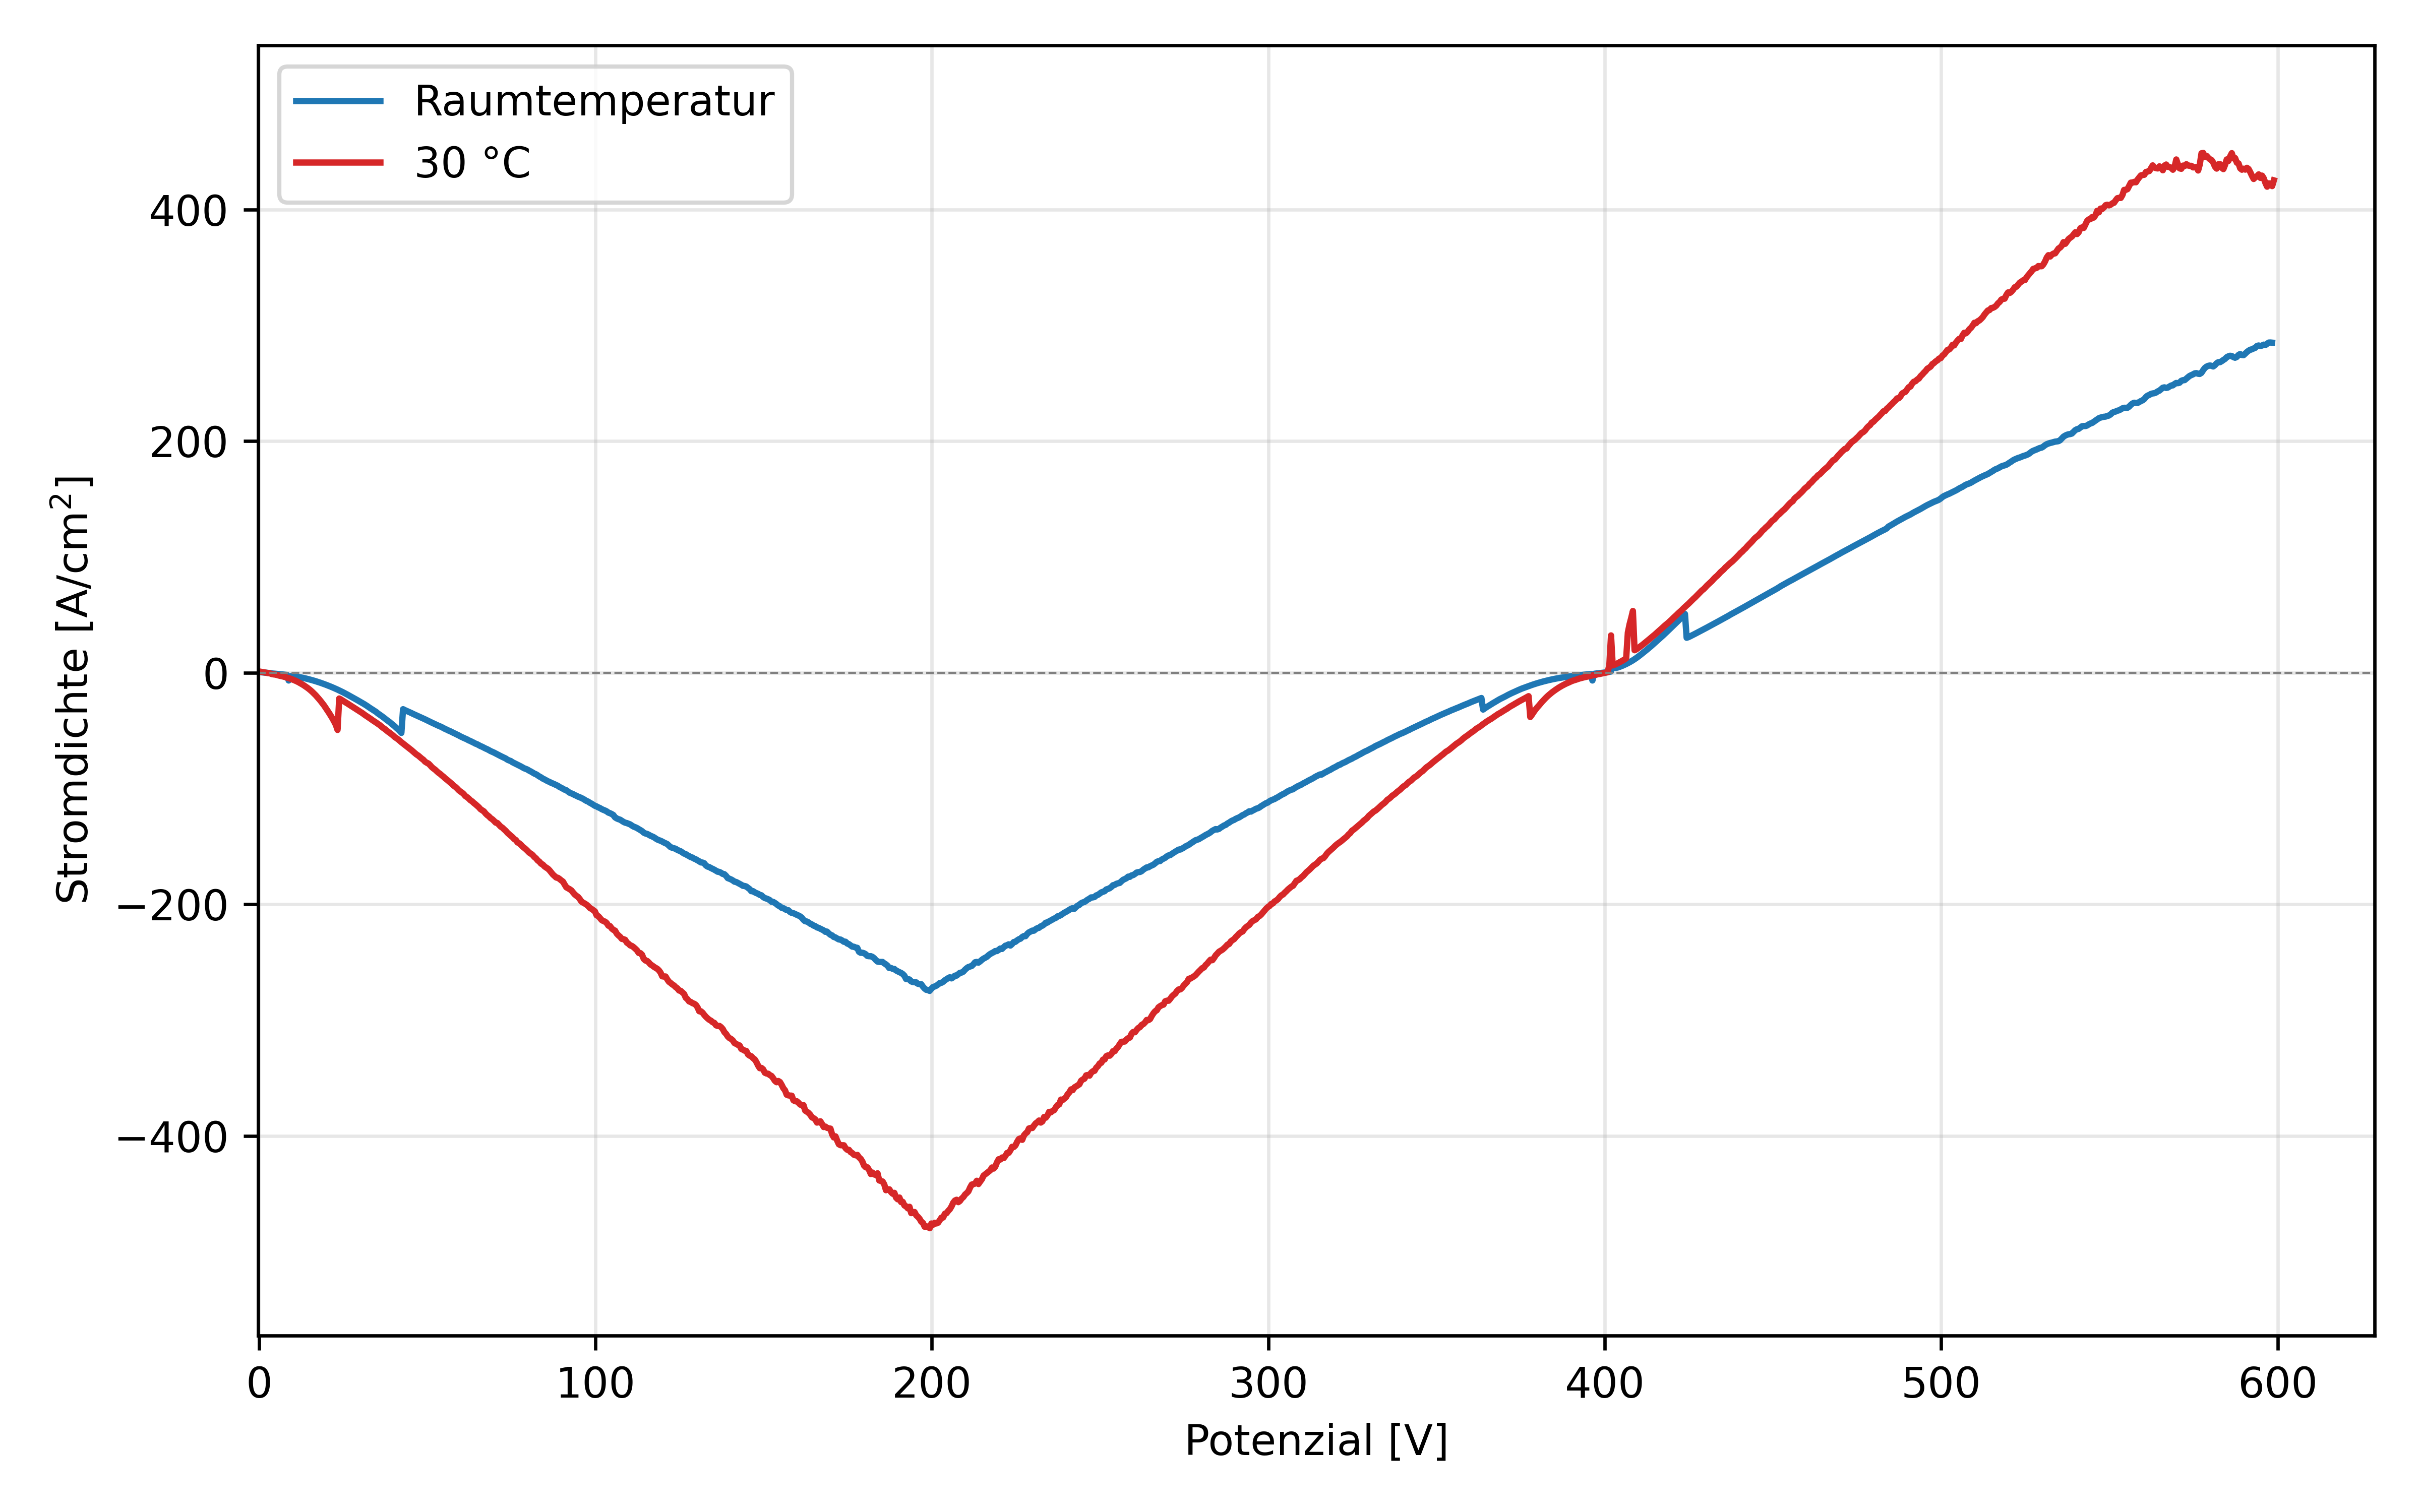
\includegraphics[width=\textwidth]{EIsen_in_H2So4_Vergleich.png} % Dateinamen anpassen!
        \caption*{B) \& C) Fe in verd.\ $\text{H}_2\text{SO}_4$ bei RT und $\qty{30}{\celsius}$}
        \label{fig:plot_BC}
    \end{subfigure}
    
    \caption{Stromdichte-Potenzial-Kurven der verschiedenen Halbzellen-Systeme}
    \label{fig:stromdichte_kurven}
\end{figure}

\noindent Die aufgezeichneten Graphen (Abb. \ref{fig:stromdichte_kurven}) lassen sich grundlegend in zwei Bereiche unterteilen: Die Abschnitte mit negativer Stromdichte repräsentieren den \textbf{kathodischen Teilstrom}. Hier findet am Metall eine Reduktion statt. Die Abschnitte mit positiver Stromdichte entsprechen hingegen dem \textbf{anodischen Teilstrom}, bei dem das Metall oxidiert wird und aktiv in Lösung geht. Der exakte Nulldurchgang der Kurve (Stromdichte $i = 0$) kennzeichnet das Korrosions- beziehungsweise Ruhepotenzial. An diesem Punkt heben sich der anodische und der kathodische Teilstrom betragsmäßig exakt auf.

\noindent Für Eisen in verdünnter Schwefelsäure \textbf{(B \& C)} zeigt sich nach dem Nulldurchgang ein steiler Anstieg des anodischen Teilstroms. Der direkte Temperaturvergleich belegt, dass die Kurve bei \qty{30}{\celsius} sowohl im anodischen als auch im katholischen Bereich betragsmäßig steiler verläuft als bei Raumtemperatur. Diese Beobachtung lässt sich dadurch erkl\"aren, dass die Temperaturerhöhung  zusätzliche thermische Energie liefert, wodurch die Aktivierungsenergie für den Ladungsdurchtritt leichter überwunden wird. Dies beschleunigt nicht nur die Eisenauflösung (anodischer Teilstrom), sondern auch die Reduktion der Protonen zu Wasserstoffgas (kathodischer Teilstrom).

\noindent Ein anderes Verhalten zeigt der legierte Chromstahl in Schwefelsäure \textbf{(D)}. Hier verbleibt der Graph nach dem Erreichen der Nulllinie für längere Zeit auf diesem Null-Niveau (Stromdichte $i \approx 0$), obwohl die Messung fortschreitet. Dieses Verweilen auf der Nulllinie ist der charakteristische \textbf{Passivierungsbereich}. Es bedeutet, dass das zulegierte Chrom an der Oberfl\"ache oxidiert und spontan eine extrem dichte, festhaftende Passivschicht (Chromoxid) ausbildet. Diese Schicht wirkt als Barriere, isoliert das darunterliegende Metall vom Elektrolyten und blockiert den anodischen Ladungsdurchtritt nahezu vollständig. Erst mit steigendem Potential wird diese bricht diese Schicht durchbrochen, wodurch die Stromdichte schlagartig wieder ansteigt.

\noindent Bei reinem Eisen in Kochsalzlösung \textbf{(A)} verläuft die Kurve nach dem Nulldurchgang ebenfalls flach an der Nulllinie entlang, bevor der anodische Teilstrom ansteigt. Hierbei kommt es zu einer kinetische Hemmung durch die Bildung einer porösen Schicht (Rost). Diese Schicht bremst den Stofftransport ab, kann das Metall aber nicht dauerhaft vor weiterer Korrosion schützen. Der Abfall der Stromdichte am Ende der Messung l\"asst sich auf Messfehler des Messger\"ats zur\"uckf\"uhren und konnte auch durch eine zweite Messung nicht eliminiert werden.
\noindent Auch lassen sich im gesamten Kurvenverlauf Ungenauigkeiten durch \"au{\ss}ere Einflussfaktoren, wie St\"o{\ss}e des Potentiostats, in Form von kleinen Ausschl\"agen der Stromdichte beobachten.
\noindent Die auf der y-Achse aufgetragene Stromdichte ($i = I/A$) h\"angt maßgeblich von der aktiven Probenfläche $A$ abhängt. Da diese Fläche bei den verwendeten Metallblechen durch die Klemmung und Benetzung im Versuchsaufbau nur grob abgeschätzt ist, unterliegen die absoluten quantitativen Messwerte einer gewissen Messunsicherheit.

%\begin{figure}[htb]
%\centering
%\includegraphics[width=0.7\textwidth]{färbungKRMZ.jpeg}
%\caption{F\"arbung im Hauptgef\"a{\ss} w\"ahrend der Messung} 
%\label{fig:MZfarbung}
%\end{figure}
%
%W\"ahrend der Messung \textbf{C)} l\"asst sich eine Tr\"ubung des Hauptgef\"a{\ss}es feststellen (Abb. \ref{fig:MZfarbung})

\newpage
\section{Zusammenfassung}


Die Auswertung zeigt , dass unlegiertes Eisen in sauren Medien einer aktiven Auflösung unterliegt. Dieser Prozess wird durch die Zufuhr thermischer Energie (bei \qty{30}{\celsius}) nochmals beschleunigt. Auch in neutraler Kochsalzlösung bietet die entstehende poröse Rostschicht keinen dauerhaften Schutz, sondern bewirkt lediglich eine temporäre kinetische Hemmung. Im  Kontrast dazu l\"asst sich das Prinzip der Passivierung am legierte Chromstahl beobachten.

\noindent Um den globalen Korrosionskosten zukünftig noch effektiver zu begegnen, geht die moderne Werkstoffforschung über die klassischen Passivierungseffekte hinaus. Aktuelle Entwicklungen befassen sich mit korrosionsbest\"andiger Materialien . Beispielsweise die selbstheilende Beschichtungen (Self-Healing Coatings) \cite{zhang2018self}. Diese enthalten Mikrokapseln mit Korrosionsinhibitoren, die bei einer mechanischen Verletzung der Oberfläche aufreißen und die Fehlstelle autonom versiegeln, bevor der elektrochemische Abbau des Metalls beginnen kann. 

\noindent Darüber hinaus revolutionieren sogenannte Hochentropie-Legierungen (High-Entropy Alloys) das klassische Legierungsdesign \cite{liang2024corrosion}. Sie bestehen mehreren Elementen zu fast gleichen atomaren Anteilen, was zu einer gro{\ss}en thermodynamischen Stabilität und einer starken Korrosionsbeständigkeit f\"uhrt. 

\newpage
\appendix
\section{Anhang}

\newpage
\section{Literaturverzeichnis}

\bibliography{korrosionbib}
\bibliographystyle{IEEEtran}

\end{document}
